\documentclass[14pt]{extbook}
\usepackage{multicol, enumerate, enumitem, hyperref, color, soul, setspace, parskip, fancyhdr} %General Packages
\usepackage{amssymb, amsthm, amsmath, bbm, latexsym, units, mathtools} %Math Packages
\everymath{\displaystyle} %All math in Display Style
% Packages with additional options
\usepackage[headsep=0.5cm,headheight=12pt, left=1 in,right= 1 in,top= 1 in,bottom= 1 in]{geometry}
\usepackage[usenames,dvipsnames]{xcolor}
\usepackage{dashrule}  % Package to use the command below to create lines between items
\newcommand{\litem}[1]{\item#1\hspace*{-1cm}\rule{\textwidth}{0.4pt}}
\pagestyle{fancy}
\lhead{Progress Quiz 10}
\chead{}
\rhead{Version A}
\lfoot{}
\cfoot{}
\rfoot{Fall 2020}
\begin{document}

\begin{enumerate}
\litem{
Simplify the expression below into the form $a+bi$. Then, choose the intervals that $a$ and $b$ belong to.\[ \frac{63 - 33 i}{8 - i} \]\begin{enumerate}[label=\Alph*.]
\item \( a \in [537, 537.06] \text{ and } b \in [-3.5, -1] \)
\item \( a \in [7.74, 7.89] \text{ and } b \in [32.5, 34] \)
\item \( a \in [8.2, 8.52] \text{ and } b \in [-201.5, -199.5] \)
\item \( a \in [7.19, 7.49] \text{ and } b \in [-6, -4] \)
\item \( a \in [8.2, 8.52] \text{ and } b \in [-3.5, -1] \)

\end{enumerate} }
\litem{
Simplify the expression below into the form $a+bi$. Then, choose the intervals that $a$ and $b$ belong to.\[ (-10 - 8 i)(4 + 6 i) \]\begin{enumerate}[label=\Alph*.]
\item \( a \in [-41, -39] \text{ and } b \in [-48, -47] \)
\item \( a \in [-93, -87] \text{ and } b \in [-34, -23] \)
\item \( a \in [-93, -87] \text{ and } b \in [22, 34] \)
\item \( a \in [8, 14] \text{ and } b \in [90, 93] \)
\item \( a \in [8, 14] \text{ and } b \in [-98, -82] \)

\end{enumerate} }
\litem{
Simplify the expression below and choose the interval the simplification is contained within.\[ 13 - 2 \div 1 * 19 - (17 * 14) \]\begin{enumerate}[label=\Alph*.]
\item \( [-265, -259] \)
\item \( [-594, -583] \)
\item \( [247.89, 253.89] \)
\item \( [-225.11, -224.11] \)
\item \( \text{None of the above} \)

\end{enumerate} }
\litem{
Choose the \textbf{smallest} set of Complex numbers that the number below belongs to.\[ \sqrt{\frac{0}{625}}+\sqrt{8}i \]\begin{enumerate}[label=\Alph*.]
\item \( \text{Nonreal Complex} \)
\item \( \text{Pure Imaginary} \)
\item \( \text{Irrational} \)
\item \( \text{Rational} \)
\item \( \text{Not a Complex Number} \)

\end{enumerate} }
\litem{
Choose the \textbf{smallest} set of Real numbers that the number below belongs to.\[ -\sqrt{\frac{61009}{361}} \]\begin{enumerate}[label=\Alph*.]
\item \( \text{Irrational} \)
\item \( \text{Not a Real number} \)
\item \( \text{Integer} \)
\item \( \text{Rational} \)
\item \( \text{Whole} \)

\end{enumerate} }
\end{enumerate}

\end{document}\documentclass[14pt]{extbook}
\usepackage{multicol, enumerate, enumitem, hyperref, color, soul, setspace, parskip, fancyhdr} %General Packages
\usepackage{amssymb, amsthm, amsmath, bbm, latexsym, units, mathtools} %Math Packages
\everymath{\displaystyle} %All math in Display Style
% Packages with additional options
\usepackage[headsep=0.5cm,headheight=12pt, left=1 in,right= 1 in,top= 1 in,bottom= 1 in]{geometry}
\usepackage[usenames,dvipsnames]{xcolor}
\usepackage{dashrule}  % Package to use the command below to create lines between items
\newcommand{\litem}[1]{\item#1\hspace*{-1cm}\rule{\textwidth}{0.4pt}}
\pagestyle{fancy}
\lhead{Progress Quiz 10}
\chead{}
\rhead{Version A}
\lfoot{}
\cfoot{}
\rfoot{Fall 2020}
\begin{document}

\begin{enumerate}
\litem{
Write the equation of the line in the graph below in Standard form $Ax+By=C$. Then, choose the intervals that contain $A, B, \text{ and } C$.
\begin{center}
    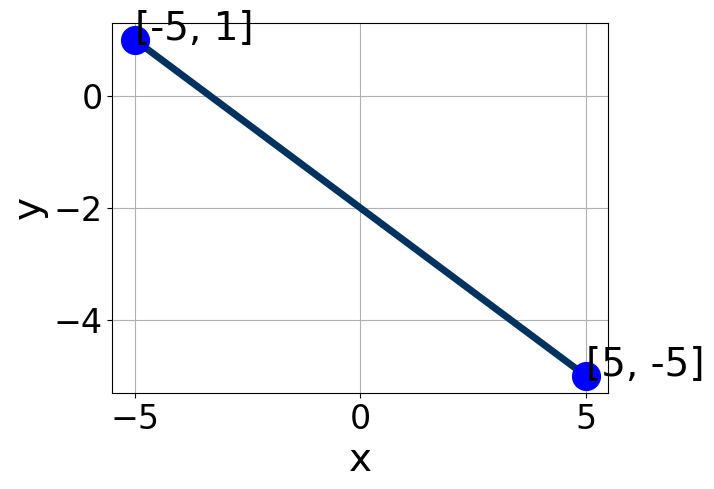
\includegraphics[width=0.5\textwidth]{../Figures/linearGraphToStandardA.png}
\end{center}
\begin{enumerate}[label=\Alph*.]
\item \( A \in [1.16, 2.36], \hspace{3mm} B \in [-10.4, -4.2], \text{ and } \hspace{3mm} C \in [20, 27] \)
\item \( A \in [1.16, 2.36], \hspace{3mm} B \in [1.9, 7.4], \text{ and } \hspace{3mm} C \in [-30, -22] \)
\item \( A \in [-0.06, 0.68], \hspace{3mm} B \in [-0.1, 2.6], \text{ and } \hspace{3mm} C \in [-6, -1] \)
\item \( A \in [-0.06, 0.68], \hspace{3mm} B \in [-2.7, 0.2], \text{ and } \hspace{3mm} C \in [5, 7] \)
\item \( A \in [-2.04, -1.17], \hspace{3mm} B \in [-10.4, -4.2], \text{ and } \hspace{3mm} C \in [20, 27] \)

\end{enumerate} }
\litem{
Find the equation of the line described below. Write the linear equation as $ y=mx+b $ and choose the intervals that contain $m$ and $b$.\[ \text{Parallel to } 4 x + 7 y = 13 \text{ and passing through the point } (4, 2). \]\begin{enumerate}[label=\Alph*.]
\item \( m \in [-1.5, -0.39] \hspace*{3mm} b \in [-2.4, -1.5] \)
\item \( m \in [-1.5, -0.39] \hspace*{3mm} b \in [-4.5, -3.5] \)
\item \( m \in [-1.5, -0.39] \hspace*{3mm} b \in [3.1, 4.4] \)
\item \( m \in [-1.94, -0.9] \hspace*{3mm} b \in [3.1, 4.4] \)
\item \( m \in [0.46, 1.54] \hspace*{3mm} b \in [-1.8, 0.4] \)

\end{enumerate} }
\litem{
First, find the equation of the line containing the two points below. Then, write the equation as $ y=mx+b $ and choose the intervals that contain $m$ and $b$.\[ (4, 11) \text{ and } (-8, -5) \]\begin{enumerate}[label=\Alph*.]
\item \( m \in [1.33, 2.33] \hspace*{3mm} b \in [2.52, 3.55] \)
\item \( m \in [1.33, 2.33] \hspace*{3mm} b \in [3.97, 6.69] \)
\item \( m \in [-2.33, 0.67] \hspace*{3mm} b \in [-16.17, -13.14] \)
\item \( m \in [1.33, 2.33] \hspace*{3mm} b \in [6.99, 8.18] \)
\item \( m \in [1.33, 2.33] \hspace*{3mm} b \in [-6.38, -4.67] \)

\end{enumerate} }
\litem{
Solve the equation below. Then, choose the interval that contains the solution.\[ -2(-8x -19) = -5(-6x + 12) \]\begin{enumerate}[label=\Alph*.]
\item \( x \in [-0.9, -0.57] \)
\item \( x \in [-1.33, -0.99] \)
\item \( x \in [5.2, 5.7] \)
\item \( x \in [-9.77, -9.41] \)
\item \( \text{There are no real solutions.} \)

\end{enumerate} }
\litem{
Solve the linear equation below. Then, choose the interval that contains the solution.\[ \frac{4x + 9}{8} - \frac{-8x -9}{7} = \frac{3x -9}{4} \]\begin{enumerate}[label=\Alph*.]
\item \( x \in [-2.1, 0.3] \)
\item \( x \in [-6, -4.8] \)
\item \( x \in [-2.4, -1.7] \)
\item \( x \in [-31.3, -28.9] \)
\item \( \text{There are no real solutions.} \)

\end{enumerate} }
\end{enumerate}

\end{document}